
\section{Bayesian Neural PBC}

\subsection{Simple Pendulum}

The equation of motion of a simple pendulum with measurement noise is given by
%
\begin{equation}
    \dd x = \bmat{
        \dot{\vartheta} \\ 
        a \sin{\vartheta} + u^\theta(x)
    } \dd t+ \nabla_x u^\theta(x) \dd W_t,
    \label{eq:pendulum_sde}
\end{equation}
%
where $a=mgl/I$, $\dd W_t$ is the Wiener process, $x = (\vartheta,
\dot{\vartheta})$ is the state of the pendulum where $\vartheta = 0$ corresponds
to the upright position, and the control input $u$ is the torque generated by
the actuator. 
%
The torque \(u^\theta\) is limited by \(\abs{u} \leq u_{\textrm{max}}\).
%
The maximum torque $u_{\textrm{max}}$ available is such that the upward
equilibrium point cannot be reached by just rotating in one direction, as the
gravitational force overcomes the motor torque eventually. The controller has to
be clever enough to overcome gravitational forcing with a combination of
built-up momentum and torque bandwidth.

The objective of this case study is to stabilize the homoclinic orbit of the
pendulum whose single parameter $a$ has the nominal value $9.81$
\unit{$s^{-2}$}. To this end, we learn a target function that directly
parameterizes the controller $u^\theta$.

\subsubsection{Training} 
Algorithm~\ref{algo:nbl} is carried out with expert
trajectories generated by the vanilla energy-shaping control
(ESC)~\cite{underactuated}. The ESC takes the general form
%
\begin{equation}
    u^\theta(\vartheta, \dot{\vartheta}; \theta) = \theta_1 \dot{\vartheta} + \theta_2 \cos{(\vartheta)} \dot{\vartheta} + \theta_3 \dot{\vartheta}^3,
    \label{eq:pendulum_esc}
\end{equation}
%
where the weights $\{\theta_i\}_{i=1}^3$ satisfy $-\theta_1 = \theta_2 = 2a
\theta_3 < 0$ in the vanilla ESC. 

The running cost function is chosen to be the loss $J_{track}(\gamma_\bot)$
from homoclinic orbit $\gamma^\star$ provided in~\eqref{eq:xperploss}; the
corresponding likelihood is given by~\eqref{eq:track_likelihood}. We collect
dataset $\mathcal{D}$ of initial states sampled from the expert trajectory,
per the state sampling technique discussed in
Section~\ref{ssec:state_sampling}. For this particular experiment, we use
Hamiltonian Monte Carlo outlined in Algorithm~\ref{algo:hmc} to infer the
exact posterior distribution $p(\theta | \mathcal{D})$. We compare the
Bayesian policy inferred from the procedure in Algorithm~\ref{algo:nbl} with
the deterministic policy, which is simply given by the point-estimates of
the expert vanilla ESC in~\eqref{eq:pendulum_esc}~\cite{acc}.

\subsubsection{Simulation Tests} 
The homoclinic orbit of the pendulum is defined by the $2a$-level set of the
total energy $\mathcal{H} = \nicefrac{1}{2}\dot{\vartheta}^2 + a(1 +
\cos{\vartheta})$. Hence, an appropriate measure of the distance to the
homoclinic orbit is given by the absolute value $\bigl| \mathcal{\tilde{H}}
\bigr|$ of the error: $\mathcal{\tilde{H}} = \mathcal{H} - 2a$. We evaluate the
performance of a closed-loop system by recording the value $\zeta = \min \,
\bigl| \mathcal{\tilde{H}} \bigr|$, where the minimum is taken over the last $2$
seconds of a $10$-second-long trajectory.


We demonstrate the robustness of the Bayesian policy by comparing $\zeta$,
as a function of the system parameter $a$, with that of the deterministic
policy.
%
We also investigate the effects of the prior distribution of $\theta$ on the
performance of the controllers.
%
In particular, we examine a uniform prior and a Gaussian prior centered around
the deterministic solution of~\eqref{eq:pendulum_esc}.
%
The comparisons between the controllers from both cases are shown in
Figure~\ref{fig:bayes_compare}.
%

In addition to uncertainties in $a$, we test the deterministic and Bayesian
policies with measurement noise, modelled as a Wiener process with variance
$0.0005$ \unit{rad} in the $\vartheta$- and $0.05$ \unitfrac{rad}{s} in the
$\dot{\vartheta}$-directions.
%
These numbers are chosen to represent a typical error arising from an
optical encoder with a resolution of 2048 pulses per revolution and its naive
differentiation via backward difference.
%
To capture the influence of measurement noise, we generate 20 trajectories
by integrating~\eqref{eq:pendulum_sde} from the same initial states. 
%
These trajectories are then used to compute $\zeta$. 
%
The effects of noise on $\zeta$ are reflected by the error bands in
Figure~\ref{fig:bayes_compare}.

The results show that Bayesian learning yields controllers that outperform 
their deterministic counterpart throughout the whole range of $a$.
%
The marginalization method in~\eqref{eqn:marginalization} for selecting $\theta$
from the learned distribution performs best when a uniform prior is used, while
the MAP method performs best with the Gaussian prior.
%
We emphasize that the error bands of the marginalized and MAP point
estimates stay well below those of the deterministic curve in the top plot of
Figure~\ref{fig:bayes_compare}.
%
This implies that the controllers produced by Bayesian learning perform
consistently better than the deterministic controller, demonstrating their
robustness against model uncertainty and measurement noise.


\begin{figure}[tb]
    \centering
    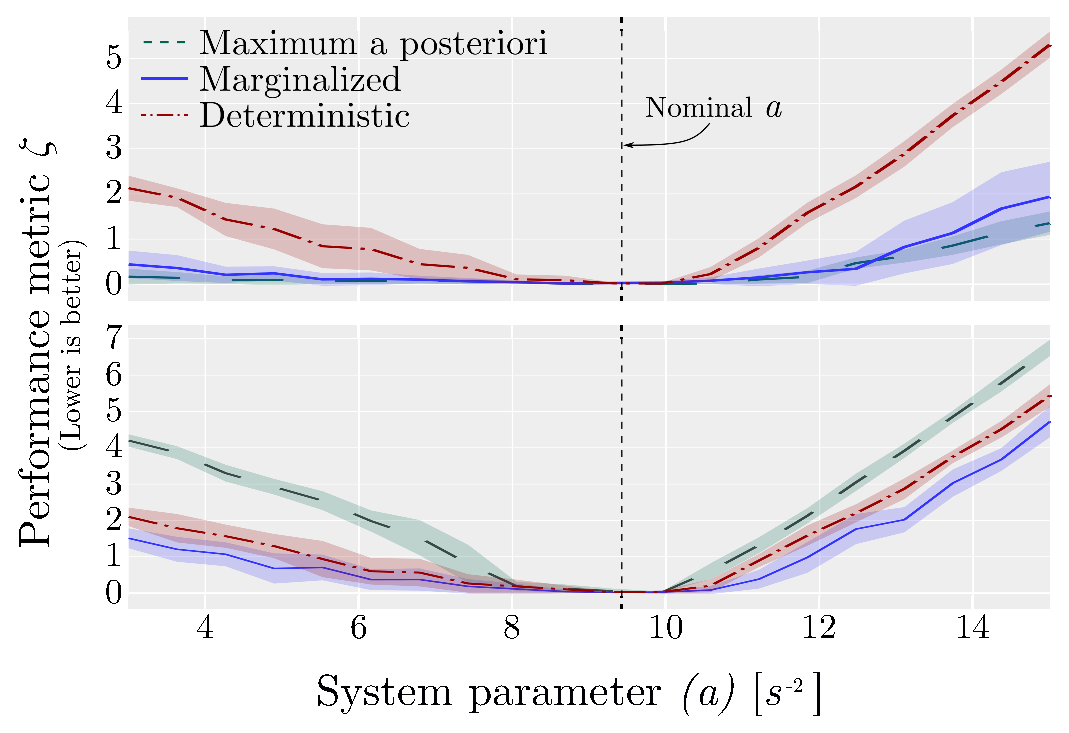
\includegraphics[width=0.7\linewidth]{figures/H_combined.eps}
    \caption{
        Performance comparisons between deterministic and Bayesian learning
        methods. 
        %
        The training is initialized with a Gaussian prior (top), and a
        uniform prior (bottom). 
        %
        The continuous error band is generated by computing $\zeta$ from 20
        trajectories of~\eqref{eq:pendulum_sde}, starting at the downward
        equilibrium with a small disturbance. 
        %
        The solid lines represent the mean of $\zeta$. 
        %
        Best viewed in color.
        %
    }
    \label{fig:bayes_compare}
\end{figure}

\subsection{Inertia Wheel Pendulum}
\label{subsec:iwp}

The IWP mechanism consists of a pendulum with an actuated wheel instead of a static
mass.
%
The wheel has mass $m$, which is connected to a massless rod of length \(l\). 
%
The position of the rod is denoted by the angle \(q_1\) measured with
respect to the downward vertical position.
%
The position of the wheel \(q_2\) is measured with respect to the vertical
line through the center of the wheel.

The Hamiltonian of the IWP is given by Equation ~\eqref{eq:system_hamiltonian}
with $n=2$ and
%
\begin{equation*}
    M = \bmat{I_1 & 0 \\ 0 & I_2},
    \;
    G = \bmat{-1 \\ \phantom{-}1},
    \;
    V(q) = mgl \left( \cos q_1 - 1 \right),
\end{equation*}
%
and $p = \left(I_1 \dot{q}_1,I_2 \dot{q}_2\right)$. 
%
We denote the state of the system as $x = (q_1, q_2, \dot{q}_1, \dot{q}_2)$.
%
The parameters \(I_1\) and \(I_2\) denote the moment of inertia of the pendulum
and the wheel, respectively, and \(g\) is the gravitational constant.
%
The equations of motion of the IWP can be written as 
%
\begin{equation}
    \dd x = \bmat{\dot{q}_1 \\ \dot{q}_2 \\ \dfrac{mgl \sin(q_1) - u^\theta - b_1\dot{q}_1}{I_1} \\ \dfrac{u^\theta - b_2 \dot{q}_2}{I_2}} \dd t + \nabla_x u^\theta(x) \dd W_t, 
    \label{eq:iwp_dynamics}
\end{equation}
%
where the control input \(u^\theta\) is the torque applied to the inertia wheel
and $\{b_i\}_{i=1}^2$ are friction coefficients.
%
The desired equilibrium $x^\star$ is the origin, which corresponds to the upward
position.
%
The nominal system parameters are estimated to be $I_1 = 0.0455$ kg-m$^2$, $I_2
= 0.00425$ kg-m$^2$, and $mgl = 1.795$ N-m. 
%
% The control objective is to ensure that closed-loop trajectories
% of~\eqref{eq:iwp_dynamics} passes through a neighborhood of $x^\star$,
% at which point a linear stabilizing controller can be employed to asymptotically
% stabilize the system at $x^\star$.
%

\begin{figure}[t]
    \centering
    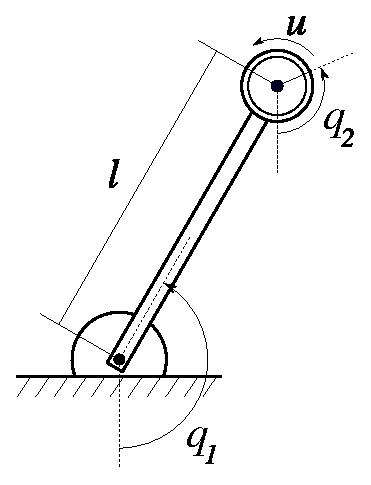
\includegraphics[width=0.25\linewidth]{figures/iwp.eps}
    \caption{Schematic of the inertia wheel pendulum. Only the joint $q_2$ is actuated, and $q_1$ is not.}
    \label{fig:iwp}
\end{figure}

\subsubsection{Training} 

The energy-like function $H_d^\theta$ is a fully-connected neural network with
two hidden layers, each with the \textsc{Elu} activation
function~\cite{clevert2015fast}. 
%
% There are, in total, 137 parameters to learn. 
% %
% They are initialized according to the Glorot
% (Xavier)~\cite{glorot2010understanding} scheme.
%
% The objective of the optimization problem~\eqref{eq:neural_pbc_finite_optim}
% consists of $\ell_{\textrm{set}}$ given by Equation~\eqref{eq:set_distance},
% with the set $\mathcal{S}$ chosen as a ball of radius $r = 0.01$ around
% $x^\star$ in the standard norm topology.
%
A uniform distribution in $[-2\pi, 2\pi] \times [-2\pi, 2\pi] \times [-10, 10]
\times [-10, 10]$ is chosen as the probability distribution from which samples
of initial states $x_0$ are drawn for the \textsc{DAgger} strategy.
%
In each gradient descent step, we sample a batch of 4 initial states
$\{x_0\}$ from $x_0 \sim \mathcal{N}(x^\star, \Sigma_0)$ and \textsc{DAgger}
as discussed in Section~\ref{ssec:state_sampling}; these initial states are
integrated forward with a time horizon of $t \in [0,3]$ seconds. 
%
In the Bayesian framework, the standard deviations $\sigma_{\zeta}$ of system
parameters $\zeta = [I_1, I_2, mgl]$ are chosen to be $10\%$ of the nominal system
parameters given in Section~\ref{sec:iwp}.
%
Moreover, we train on trajectories per the SDE
in~\eqref{eq:neural_bayesian_inference} with measurement error represented
by Wiener process with standard deviation of 0.001 and 0.02 on the joint
angles and velocities, respectively.
%
% In each gradient descent step, a batch of 4 initial conditions $\{x_0\}$
% generated by \textsc{DAgger} is integrated forward with using the Tsitouras
% $5(4)$ Runge-Kutta solver with a time horizon of $t \in [0,3]$ seconds. 
%
% The cost function is then computed and back-propagated using the
% AD-assisted adjoint method implemented in
% \verb|DiffEqFlux.jl|~\cite{DBLP:journals/corr/abs-2001-04385}.
% %
% In the Bayesian learning framework, we draw samples from the posterior and
% back-propagate through the gradients of the \textsc{Elbo} using the
% \textsc{ADVI}~\cite{kucukelbir2015automatic} scheme provided in
% \verb|Turing.jl|~\cite{turing}. 
%

We use variational inference to estimate a Gaussian posterior distribution
over uncorrelated parameters. The trainings are terminated when the loss
function $J(\gamma) = J_{set}(\gamma) + J_T(\gamma)$ and the \textsc{Elbo}
converge for the deterministic and Bayesian trainings, respectively.
%
The hyperparameters for the deterministic and Bayesian \textsc{NeuralPbc}
trainings are shown in Table~\ref{tab:training_setup_neuralpbc}.
%
It can be seen that the Bayesian training effectively learns with smaller
neural network size than the deterministic training.
\begin{table}[tb]
    \centering
    \caption{\textsc{NeuralPBC} training setup for deterministic and Bayesian frameworks}
    % \rowcolors{2}{}{Wheat1}
    \begin{tabular}{lcc}
    \toprule
    %   & \multicolumn{2}{c}{Framework} \\
    %   \cmidrule(lr){2-3}
    & Deterministic & Bayesian \\
    \midrule
        $H_d$ neural net size & (6, 12, 3, 1) & (6, 5, 3, 1)\\
        Learned parameters & 133 & 128  \\
        Optimizer & \textsc{ADAM} & DecayedAdaGrad\\
        Initial learning rate & 0.001 & 0.01\\
        Replay buffer size & 400 & 50\\
    \bottomrule
    \end{tabular}
    \label{tab:training_setup_neuralpbc}
\end{table}

\subsubsection{Simulation Tests} 
The performance of the controllers obtained from the deterministic and Bayesian
trainings are compared as follows.
%
We evaluate the performance of both trainings with parameter uncertainties
on $I_1, I_2$ and $mgl$. 
%
We introduce these uncertainties by moving the average
system parameters by $\pm 10\%$ to $\pm 50\%$ with increments of $10\%$. 
%
For each average system parameter, we sample uniformly with a $\pm 5\%$ support
around the average system parameters. 
%
This helps test the performance of the controller with various combinations of
$I_1, I_2$ and $mgl$.
%
On top of the system parameter uncertainties, we introduce measurement noise
represented by a Wiener process with standard deviation of $0.001$ and $0.02$ on
the joint angles and velocities, respectively. 
%
Figure~\ref{fig:comparison_neuralpbc} shows the performance of deterministic and
Bayesian trainings using an accumulated quadratic loss of the form
\begin{equation} J^T = \frac{1}{2}\int_0^T \left(x^\top Qx + u^\top Ru \right) dt.
\label{eq:performance_metric} \end{equation}
%
The controller learned from the Bayesian training is marginalized over 10
parameters sampled from the posterior.
As seen in Figure~\ref{fig:comparison_neuralpbc}, the Bayesian training
effectively collects less cost for large error in system parameters.
%
Moreover, the error band on the cost of the Bayesian training is smaller than
that of the deterministic training; this shows that the marginalized controller
is more robust against measurement noise.
%   
\begin{figure}
    \centering
    \includegraphics[clip,width=0.7\linewidth]{./figures/bandplot2.eps}%
    \caption{\textsc{NeuralPBC} Performance metric ($J^T$) for various
    error in system parameters. Measurement noise included as Wiener process
    with standard deviation of $0.001$ and $0.02$ on joint angles and
    velocities, respectively}
    \label{fig:comparison_neuralpbc}
\end{figure}

\subsubsection{Hardware Tests} 
The controllers from deterministic and Bayesian training schemes are
evaluated on hardware. 
%
We deliberately modify the hardware and test the controllers without any
additional training.
%
In particular, throughout the experiments, the inertia wheel attached to $q_2$
is replaced with parts (labelled A-C on Table~\ref{tab:modified_params}) whose
mass and inertia are different from the nominal values.
%
The modified system parameters are summarized in
Table~\ref{tab:modified_params}.
%
% The parameter error listed on the last column of Table~\ref{tab:modified_params}
% is computed by $\|p - p_{\textrm{nom}}\| / \|p_{\textrm{nom}}\|$.
\begin{table}[tb]
    \centering
    \caption{System parameters used in real-world experiments. The errors in the
    last column are $\|p_s - p^{\textrm{nom}}_{s}\| / \|p^{\textrm{nom}}_{s}\|$}.
    % \rowcolors{2}{}{Wheat1}
    \begin{tabular}{lcccc}
    \toprule
    Parameter set $p_s$ & $I_1$ & $I_2$ & $mgl$ & Error \\
    \midrule
    Nominal & 0.0455 & 0.00425 & 1.795 & 0 \\
    A & 0.0417 & 0.00330 & 1.577 & $0.122$ \\
    B & 0.0378 & 0.00235 & 1.358 & $0.243$ \\
    C & 0.0340 & 0.00141 & 1.140 & $0.365$ \\
    \bottomrule
    \end{tabular}
    \label{tab:modified_params}
\end{table}
    
The system starts from rest at the downward position. 
%
A small disturbance in the $q_1$ direction is introduced to start the swing-up.
%
The state $x$ is recorded and~\eqref{eq:performance_metric} is the
performance metric used to evaluate the controllers. The results are
summarized in Figure~\ref{fig:neuralpbc_bar_plot}.
%
\begin{figure}[t]
    \centering
    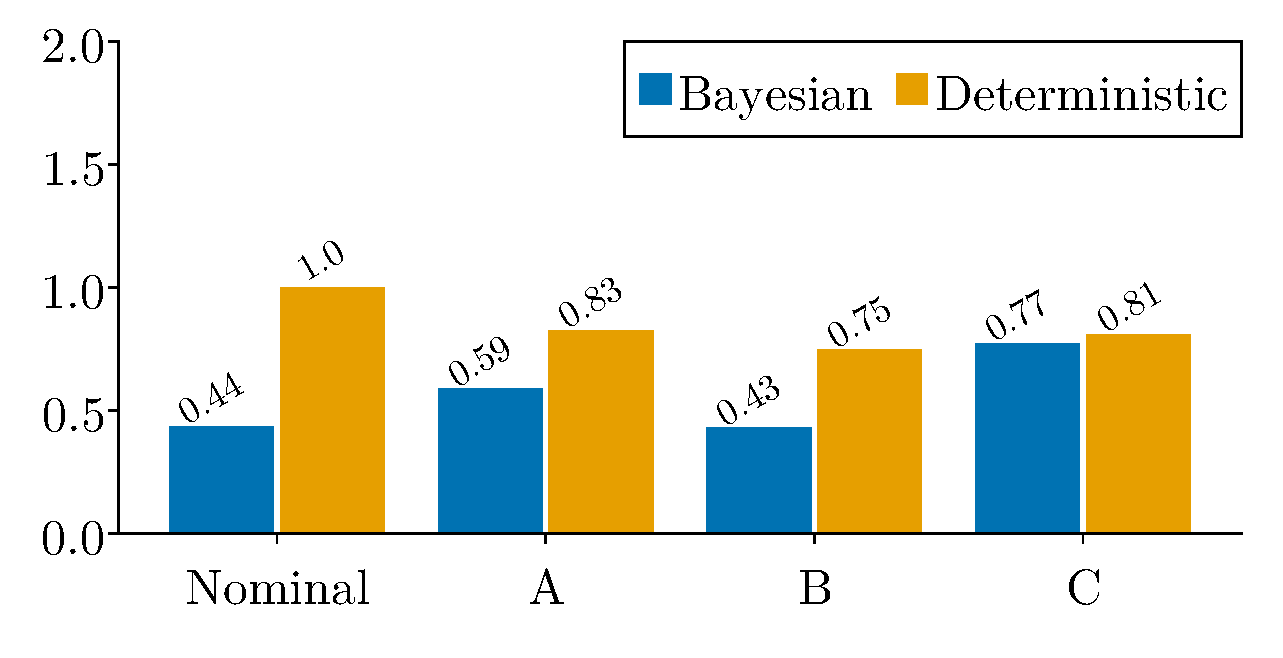
\includegraphics[width=0.6\linewidth]{./figures/pbc_bar.eps}
    \caption{
        %
        Controller performance for modified system parameters. 
        %
        The performance metric is given by
        Eq.~\eqref{eq:performance_metric}.
        %
        Lower values are better. 
        %
        These results show that controllers trained via Bayesian learning are
        consistently more robust to errors in system parameters.
        %
    }
    \label{fig:neuralpbc_bar_plot}
\end{figure}

In all scenarios, our controllers are able to achieve the control objective
despite the errors introduced in the system parameters.
%
% Furthermore, the controller from Bayesian training consistently outperforms the
% controller from deterministic training, supporting the theoretical justification
% discussed in Section~\ref{ssec:justification}. 
%
These results demonstrate that our approach enables a unified way to tackle
nonlinear control problems while simultaneously incorporating prior knowledge
and model uncertainties.
%
  
\subsection{Rimless Wheel}

